\documentclass{ECOS_2021}
%\usepackage{timesnew}
\usepackage{times}
\usepackage{graphicx}
\usepackage{amsmath}
\usepackage{amsfonts}
\usepackage{amssymb}
\usepackage{mathtools}
\usepackage{enumitem}
\usepackage{cite}
\usepackage{gensymb}
\makeatletter
\let\NAT@parse\undefined
\makeatother
\usepackage{hyperref}
\usepackage{float}

%\renewcommand{\rmdefault}{phv} % Arial
%\renewcommand{\sfdefault}{phv} % Arial

\title{\sffamily A thermodynamic and technical feasibility study of subsurface storage of energy in the North Sea abandoned reservoirs}
\rmfamily
\author{Ali A. Eftekhari$^{a}$}

%\heading{First A. Author, Second B. Author and Third C. Author}

\address{$^{a}$ Technical University of Denmark,
Lyngby,
Denmark,
aliak@dtu.dk}

\abstract{\small The oil and gas extraction from the Danish sector of the North Sea
has been declining, which will lead to the cessation of production
and abandonment (i.e., plugging of the wells and removal of the facilities).
Simultaneously, the existing and in development offshore windmills
in the North Sea will ensure the availability of abundant and cheap
electricity in the region yet fail to address the intermittent nature
of the wind resources. This paper hypothesizes that the surplus electricity
in the windy days and off-peak time can be converted to physical (compressed
hot fluids) or chemical (synthetic fuels, e.g., hydrogen, ammonia,
methanol, or methane) forms and stored in the vast space of the abandoned
oil and gas reservoirs under the North Sea. The stored energy can
be extracted and consumed as carbon-neutral fuels or be converted
back to electricity when there is a shortage of wind. This work studies
the technical and thermodynamic feasibility of offshore conversion
of electricity to physical and chemical energy sources and their storage/extraction
in/from the North Sea oil and gas reservoirs. The technical feasibility
study deals with the sufficiency of the existing infrastructures including
platforms, pipelines, and surface facilities to accommodate the process
equipment for the conversion of electricity to physical and chemical
storable forms. Several processes including nitrogen and carbon dioxide
separation from the atmosphere, electrolysis of seawater, and reduction
of CO$_{2}$ and N$_{2}$ to synthetic fuels are simulated in a commercial
process simulator. The simulation results are used for the sizing
of process equipment and the calculation of required platform area.
The thermodynamic analysis quantifies the exergy loss during the offshore
conversion, transportation, and storage/extraction of physical and chemical energy in the reservoirs based on the results of an in-house
opensource dynamic model that simulates the multi-component non-isothermal
flow of fluids in the subsurface. The results will finally estimate
the amount of wind electricity, offshore installations, and subsurface
space that is required to make Denmark self-sufficient and independent
of fossil fuels.}

\keywords{\small Exergy analysis, Electricity to fuel, energy storage, Energy transition}

\begin{document}

% \thispagestyle{empty}

\sffamily \Large \section{Introduction} \label{Introduction} 
\rmfamily \normalsize 

Wind electricity is an intermittent and volatile source of energy.
When there is no or little wind, there is not enough electricity to
match the demand; when there is too much wind, if the electricity
is not consumed immediately, it will be wasted. The Ciara storm in
February 2020, which was only partially felt in Denmark, increased
the Danish wind electricity production to 1000 Mega Watts (MW) above
consumption, i.e. 20\% higher equivalent to the average demand of
one million European citizens. There were reports of significant curtailments
up to several thousand MW from other countries in the North Sea region.
Curtailment, which means accepting less renewable electricity than
what windfarms can deliver is another word for wasted resources. It
will soon become more severe when the North Sea is hit by a technological
storm in the form of several large wind farms that are currently evaluated,
planned, and licensed \cite{GlobalOffshoreRenewable}. More importantly,
since the electricity distribution is planned based on the unavailability
of wind resources, the biomass (that is regularly switched to coal)
power plants must always be running to compensate for the shortage
of wind, thus emitting a large amount of carbon dioxide and other
pollutants. The solution is to store electricity when production is
higher than demand and consume it when demand is higher than production. 

The oil and gas extraction from the Danish sector of the North Sea
has been declining, which will lead to the cessation of production
and abandonment (i.e., plugging of the wells and removal of the facilities).
Simultaneously, the existing and in development offshore windmills
in the North Sea will ensure the availability of abundant and cheap
electricity in the region yet fail to address the intermittent nature
of the wind resources. This chapter hypothesizes that the surplus
electricity in the windy days and off-peak time can be converted to
chemical energy (synthetic fuels, i.e. hydrogen, ammonia, methanol,
or methane) forms and stored in the vast space of the abandoned oil
and gas reservoirs under the North Sea. The stored energy can be extracted
and consumed as carbon-neutral fuels for transportation or be converted
back to electricity when there is a shortage of wind. This chapter
studies the technical and thermodynamic feasibility of offshore conversion
of electricity to chemical energy sources. The technical feasibility
study deals with the sufficiency of the existing infrastructures including
platforms, pipelines, and surface facilities to accommodate the process
equipment for the conversion of electricity to chemical storable forms.
Several processes including nitrogen and carbon dioxide separation
from the atmosphere, electrolysis of seawater, and reduction of CO$_{2}$
and N$_{2}$ to synthetic fuels are simulated in Aspen Plus process
simulator. The simulation results are used for the sizing of process
equipment and the calculation of required platform area. The thermodynamic
analysis quantifies the exergy loss during the conversion of electricity
to fuel and back, and storage/extraction of chemical energy in the
reservoirs based on the results of an in-house opensource dynamic
model that simulates the multicomponent non-isothermal flow of fluids
in the subsurface.

Background and methodology 

The electricity and heat are first transferred to a storage medium
and then injected into a suitable subsurface storage space. Several
technologies based on combinations of storage media and storage space
will be studied. The storage medium can be a chemical that is made
of readily available materials with a production process that is fossil-fuel
independent \cite{eftekhariQuantifyingRoleLiquid2020} or a fluid
that can be compressed in a capped porous rock, shown schematically
in Figure 1. The main candidates for a chemical medium are ammonia,
methanol, methane, and hydrogen made of nitrogen (from the atmosphere),
hydrogen (electrolysis of water), and carbon dioxide or other carbon
sources coming from the atmosphere (known as air capture), or biomass
(plant-based carbohydrates). These energy-intensive processes will
reduce the overall efficiency of the process as shown in Figure 2.
The subsurface that is utilized for energy storage will be subject
to cyclic physical (high and low pressure and temperature during compressed
air storage and extraction) and chemical impacts that alter the chemical
and mechanical properties of the rock. The large contact area between
the porous medium and the injected fluids enhances these alterations
and often adversely affects the storage capacity and energy and fluid
loss. Leakage of fluid and heat to the surrounding strata, e.g. aquifers,
can also have negative environmental impacts, i.e. by promoting and
accelerating biochemical activities \cite{bauerImpactsUseGeological2013}.

This paper will investigate the feasibility of the alternative use
of the ``to-be-abandoned'' fields of the North Sea and their infrastructure
as a large energy storage project that can address the intermittency
of the wind energy in the North Sea region.

There are three major questions that will be answered in this work.
First, how much energy storage is needed in Denmark? Secondly, to
what extent can the subsurface storage be helpful? Thirdly, what are
the promising technologies from a technical point of view. This paper
will provide simple, reproducible, and realistic procedures and quantitative
answers to these questions.

\sffamily \large \subsection{Future energy need of Denmark} \label{Submission}
\rmfamily \normalsize

Denmark currently consumes around 100 kWh per person per day of energy
in different forms. Eftekhari \cite{eftekhari_quantifying_2020} showed
that this can be further categorized into a 30-30-40 category: 30\%
electricity, 30\% heat, and 40\% hydrocarbon fuel. Note that the hydrocarbon
consumption for electricity production is not included in the 40\%
hydrocarbon fuel. We can assume that in the future, all the warming
systems and short distance transport will be electrified; therefore,
by assuming a realistic coefficient of performance for the future
warming systems, the 30-30-40 can be roughly converted to 45-40, i.e.
a demand of 45 kWh/day electricity per person and 40 kWh/day liquid
fuel per person. This is the energy demand that I will use in the
rest of this report. As for electricity production, the current plan
is to quadruple the current electricity capacity of the wind mills
in the North Sea. Since the capacity is not equal to the actual produced
electricity (due to, e.g. technical problems, curtailment, weather
conditions, etc.) I will estimate the intermittent electricity production
of the windmills by quadrupling the current electricity production
in Denmark. The data is available from Energinet.dk website and also
as an electronic attachment to this report, including several Matlab
functions for analysis and visualizations.

Fig. \ref{fig:Current-and-future} shows the electricity supply and
demand for January 2020 (left) and January 2050 (right). We can use
the following equation to integrate the data and obtain the average
energy supply and demand over different periods of time, i.e. from
24 hours to 6 month, as shown in Fig. \ref{eq:average-energy-demand}:
\begin{equation}
\bar{E}=\frac{1}{t_{2}-t_{1}}\int_{t_{1}}^{t_{2}}E\left(t\right)dt,\label{eq:average-energy-demand}
\end{equation}
where $E(t)$ {[}MW{]} is the electricity supply or demand in the
future and $t_{1}$ {[}s{]} and $t_{2}$ {[}s{]} represent a certain
time period. The future energy supply and demand are estimated by
using the correction factor extracted from \cite{eftekhari_quantifying_2020},
e.g.
\begin{equation}
E_{future}=\lambda_{i}E_{current},\quad i=s,\,d\label{eq:demand-adjust}
\end{equation}
where $\lambda_{d}=1.5$ denotes a 50\% in electricity demand and
$\lambda_{s}=4.0$ denotes a 400\% increase of windmill capacity in
Denmark \cite{noauthor_denmark_2020,noauthor_energy_2021}. Note that
this increase will be on the offshore sector only; however, here we
assume that the overall wind energy capacity will increase by a factor
of four. The other assumption in Eq. (\ref{eq:demand-adjust}) is
that the weather (more specifically, wind) in 2050 will be similar
to the weather condition in 2020. The visualized energy supply and
demand in Fig. \ref{fig:Current-and-future} shows that periodically,
the wind electricity supply is higher or lower than the electricity
demand, creating electricity surplus and shortage, respectively. The
alternation between surplus and shortage can occur within a few hours
to few weeks. This is better visualized in Fig. \ref{fig:Average-electricity-supply}
that shows the average surplus and shortage for periods of 24 hours
to 8 months. It can be observed that after around 6 months, the average
surplus and shortage reach a constant value. This plot unveils three
critical pieces of information about the wind electricity supply and
demand in 2050: first, the average shortage of electricity is 1.6
GW, which is a large amount of power and gives an indication of the
amount of energy that needs to be stored (although sometimes the actual
power shortage is temporarily higher as shown later). The good news
is that the average electricity surplus is 2.25 GW, which is 620 MW
higher than the average electricity shortage. These two numbers, however,
serve as a constraint for the energy storage technology that is defined
by
\[
\eta_{storage}>\frac{\text{Average shortage}}{\text{Average surplus}}=0.72,
\]
i.e. the efficiency of the storage technology must be higher than
72\%.

\begin{figure}[H]
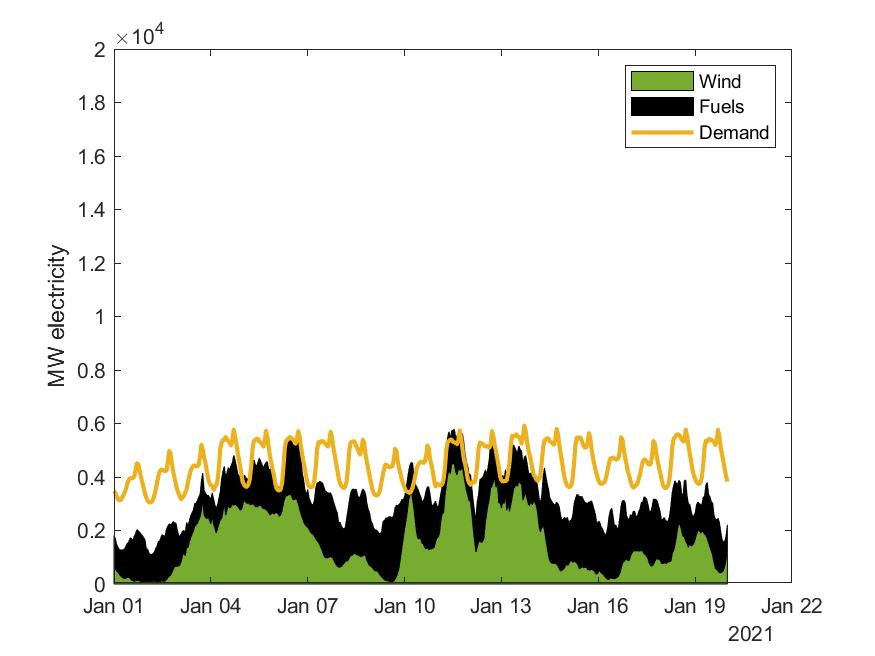
\includegraphics[width=8cm]{denmark_elec_jan2021}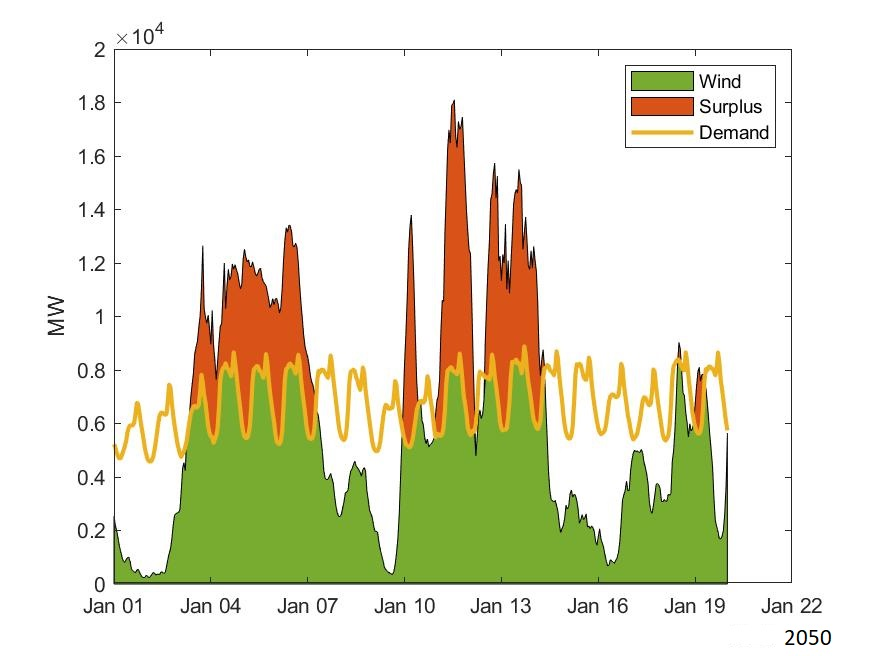
\includegraphics[width=8cm]{supply_demand_jan2050_dk}

\caption{\label{fig:Current-and-future}Current and future electricity supply
and demand of Denmark }
\end{figure}

\begin{figure}[H]
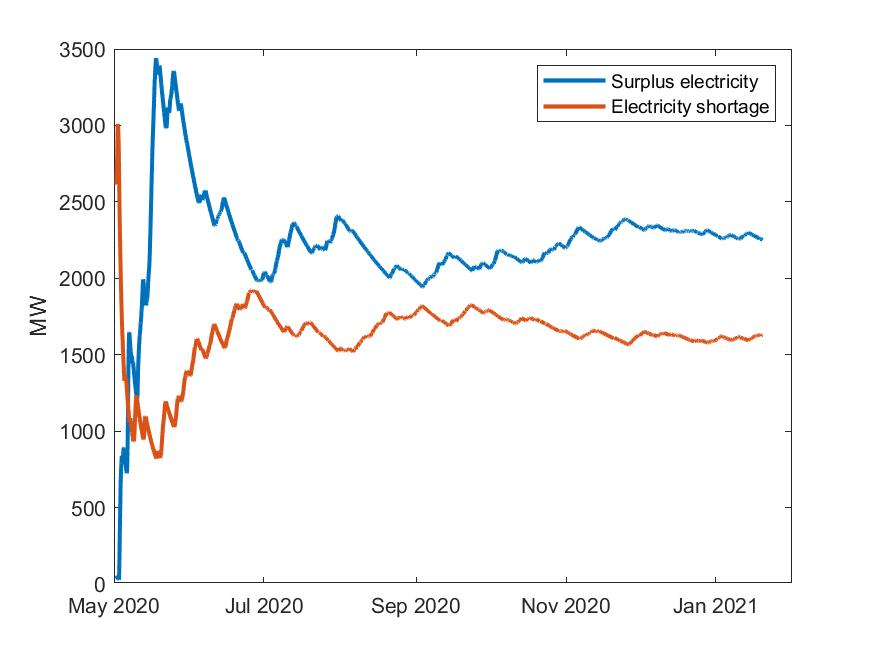
\includegraphics[width=8cm]{supply_demand_six_month_dk}

\caption{\label{fig:Average-electricity-supply}Average electricity supply
and demand for Denmark adjusted for May 2050 to January 2051; see
Eq. (\ref{eq:average-energy-demand})}
\end{figure}

Although the previous analysis provides the average storage value,
the real time electricity surplus that needs to be stored varies with
time. The same occurs with the electricity shortage, i.e. the occasional
electricity shortage can be much higher than its long-term average
value. Both of these values are shown in Fig. \ref{fig:Electricity-surplus-smooth}.
Any feasible storage process must be able to store a maximum power
surplus of 5.0 to 10.0 GW (see the peaks of the curves in Fig. \ref{fig:Electricity-surplus-smooth}-left)
and recuperate the stored power with a maximum rate of 3.0 to 6.0
GW (see the peaks of the curves in Fig. \ref{fig:Electricity-surplus-smooth}-right).
These values are critical in the design of the storage and recuperation
processes. The sizing of the required equipment and sub-processes
will be discussed in the next sections. 

\begin{figure}[H]
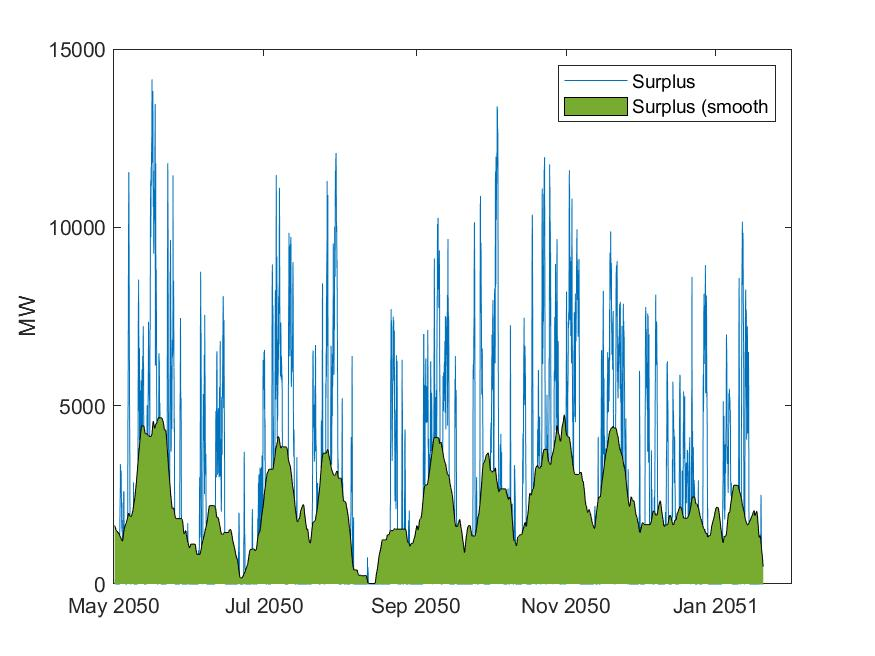
\includegraphics[width=8cm]{smoothed_surplus}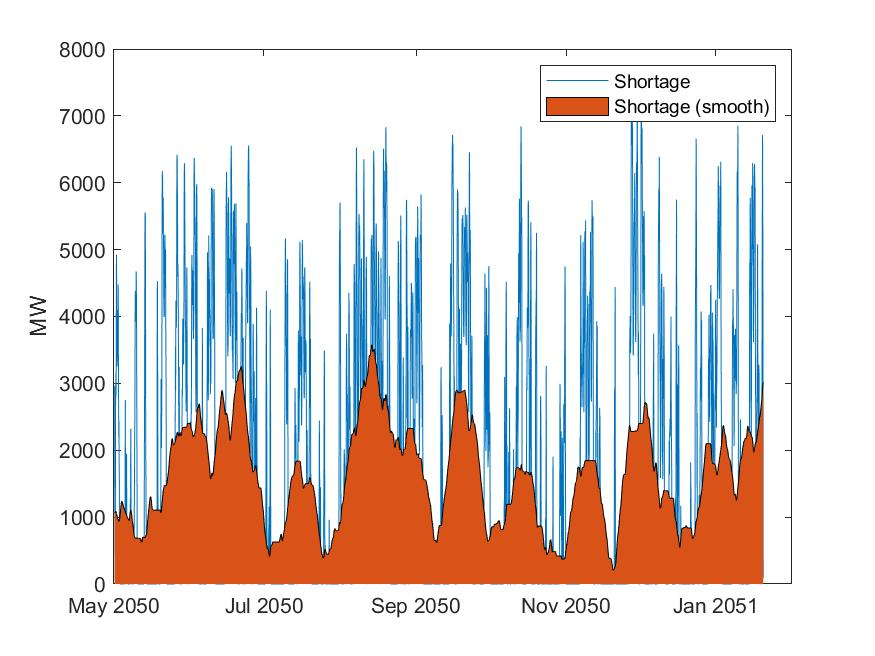
\includegraphics[width=8cm]{smoothed_deficit}

\caption{\label{fig:Electricity-surplus-smooth}Electricity surplus (left)
and shortage (right) adjusted for 2050; the smoothed curve is shown
by area plot.}
\end{figure}

We end this section by estimating the subsurface volume that is required
to store enough energy to cover for a eight month energy shortage.
Table \ref{tab:Exergy-value-efficiency} shows the exergy per unit
mole of different energy storage media that are studied in this report.
Exergy, $ex_{i}$ {[}kJ/mol{]} is the amount of energy in a system
that can be converted to mechanical work, i.e. movement or electricity.
The maximum efficiency of producing each medium, $\eta_{i}$, is also
reported in Table \ref{tab:Exergy-value-efficiency}. For these calculations,
we need to have the density of the stored fluids at reservoir conditions,
$T_{res}$ {[}K{]} and $p_{res}$ {[}bar{]}. We used the typical reservoir
conditions of the chalk fields in the Danish sector of the North Sea,
i.e. 70$^{o}$C and 200 bar. The volume of the reservoir is calculated
by
\[
V_{res,i}=\frac{\bar{E}_{shortage}t_{storage}MW_{i}}{ex_{i}\rho_{i}\varphi},
\]
where $\bar{E}_{shortage}$ {[}kW{]} is the average electricity shortage,
$t_{shortage}$ {[}s{]} is the period over which the electricity shortage
is estimated (here 8 months), $MW_{i}$ {[}kg/mol{]} is the molecular
weight of the stored fluid, $\rho_{i}$ {[}kg/m$^{3}${]} is the density
of the stored fluid at reservoir condition, and $\varphi$ {[}-{]}
is the porosity of the reservoir. Assuming a reservoir thickness of
100 m, the diameter of a chalk reservoir that can store the equivalent
of eight-month electricity shortage in 2050 is visualized in Fig.
\ref{fig:Diameter-reservoir}. The diameter is calculated assuming
an efficiency factor of one for all the energy conversions. A 2 to
3 times larger reservoir volume is required if all the efficiency
factors are included in the computations. All in all, the required
volume for the energy storage is only a small fraction of the available
reservoir volumes in the North Sea. Therefore, the reservoir volume
is not a bottleneck in the subsurface energy storage. A reservoir
with a thickness of 100 m and a radius between 100 m to 3000 m (considering
the efficiency factors) can hold enough energy to compensate for 8
months of electricity shortage in Denmark in 2050. 

\begin{table}[H]
\caption{\label{tab:Exergy-value-efficiency}Exergy value and the efficiency
of producing different energy storage media and the thermodynamic
properties at reservoir condition (70$^{o}$C, 200 bar); the efficiency
factors are only considered for the electricity to fuel conversion.}

\begin{tabular}{|c|c|c|c|c|}
\hline 
Component & $\rho$ {[}kg/m$^{3}${]} & $ex$ {[}kJ/mol{]} & $V_{res}$ {[}10$^{6}$ m$^{3}${]} & $\eta$ {[}-{]}\tabularnewline
\hline 
\hline 
NH$_{3}$ & 667.7 & 340 & 2.50 & 0.45\tabularnewline
\hline 
CH$_{4}$ & 386.6 & 831 & 1.66 & 0.36\tabularnewline
\hline 
H$_{2}$ & 67.7 & 236 & 4.21 & 0.7\tabularnewline
\hline 
CH$_{3}$OH & 871.2 & 720 & 1.70 & 0.4\tabularnewline
\hline 
Air & 733.5 & 22.0 & 59.89 & 1.0\tabularnewline
\hline 
\end{tabular}
\end{table}

\begin{figure}[H]
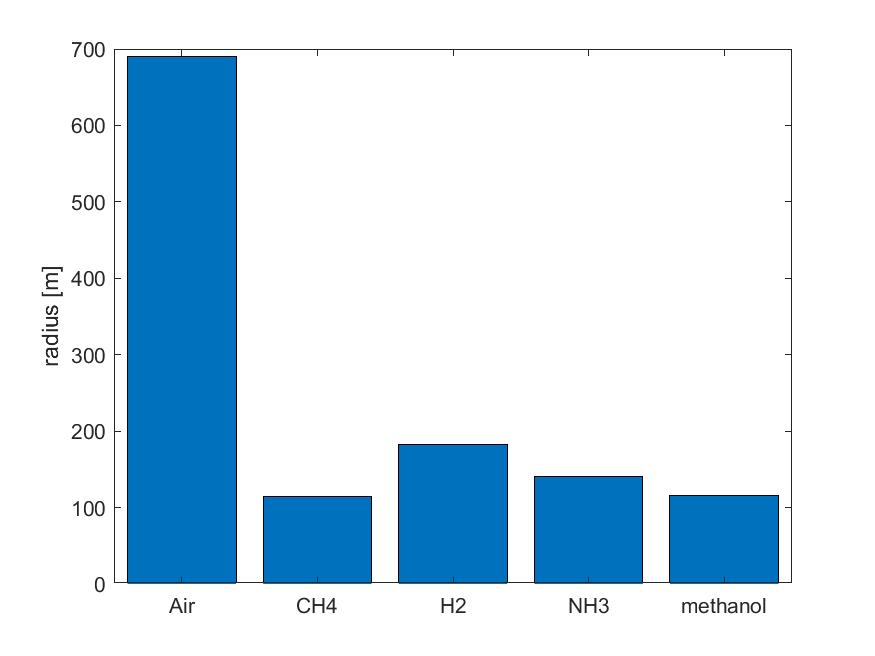
\includegraphics[width=8cm]{res_radius_8month_storage}

\caption{\label{fig:Diameter-reservoir}Diameter of a 100 m thick chalk reservoir
for the storage of fuel equivalent of 8-month electricity shortage
in 2050. All the efficiency factors are assumed to be one.}
\end{figure}

In the next chapter, several energy storage solutions will be discussed,
and a thermodynamic model will be used to compare these solutions.
The last chapter discusses the technical opportunities and limitations
of each solution. 

\sffamily \large \subsection{Information} \label{Information}
\rmfamily \normalsize 
Any doubts regarding the submission process should be sent to the organization committee contact, through the e-mail \href{mailto:ecos2020@amano.mech.waseda.ac.jp}{ecos2020@amano.mech.waseda.ac.jp}.

\sffamily \Large \section{General information about ECOS 2020 papers} \label{General}
\rmfamily \normalsize 
\sffamily \large \subsection{Manuscript preparation process} \label{Manuscript preparation process}
\rmfamily \normalsize 
The manuscript must be prepared in English (British or American spelling) and free of grammatical, spelling and/or punctuation errors. The manuscript must be thoroughly edited and proof-read before it is submitted. Authors have the responsibility to ensure clear and adequate English expression, since indecipherable language could be a valid reason for rejection of the paper.
Units in the paper must be according to the International System of Units (SI, Systme International d'Units). Other units may be given in parentheses (when they first appear in the text), dual-unit tables, or an appendix.

Authors are kindly requested to prepare the manuscript by using this template. {\bf The manuscript length is limited to twelve (12) pages at the maximum.}

The template documents contain necessary information regarding desktop publishing format, type sizes, and typefaces. Formatting styles are classified in four groups:

\sffamily \large \subsection{Manuscript submission and review process} \label{Manuscript submission and review process}
\rmfamily \normalsize 
Authors are requested to submit their manuscript, with page numbers, as Portable Document Format (PDF) file for the review process and as the \LaTeX{} file package for the ECOS Conference proceedings.

For each submission that falls within the scope of the ECOS Conference, independent experts in the field of the submission will be selected to act as reviewers. ECOS Conferences use a single-blind peer review process where the identity of the reviewers will remain anonymous\footnote{The identity of the authors will be known to the reviewers.}. The appropriate editor will assess the recommendation report from the reviewers as to whether the article should be accepted, revised or rejected. The submitted manuscript, subject to final acceptance on the basis of the reviewers report, will be included in the conference proceedings without any modifications.

\sffamily \Large \section{Organization of paper} \label{Organization of paper}
\rmfamily \normalsize
The basic parts of a paper are listed below in the order in which they should appear:

\begin{itemize}
    \item Title (Section \ref{Title}).
    \item Author(s), author's (or authors') affiliation(s), Corresponding author identifier (Section \ref{Authors information}).
    \item Abstract and Keywords (Section \ref{Abstract and keywords}).
    \item Subject matter of the paper with numbered main headings and sub-headings (Section \ref{Subject}).
    \item Acknowledgments, if any, (Section Acknowledgments).
    \item Appendices, if any, (Section Appendix A, Appendix B).
    \item Nomenclature with SI units, if any, (Section Nomenclature).
    \item References (Section References).
\end{itemize}

\sffamily \large \subsection{Title} \label{Title}
\rmfamily \normalsize
The article title appears centred at the top of the first page. To format the title authors should use the “Title” style from the formatting menu. Only the first word and proper nouns for the title should be capitalized.The  use  of  acronyms  and  abbreviations  in  the  title  should  be  avoided,  unless  they  are widely understood, or they are accompanied by the expanded expression.

\sffamily \large \subsection{Authors information} \label{Authors information}
\rmfamily \normalsize
The author's name should include first name, middle initial and
surname (e.g. Nikola Tesla, not Tesla Nikola, Ben Roethlisberger, not Roethlisberger Ben; Ming Yao, not Yao Ming). It should be written centered, in 12pt boldface Roman,
12pt below the title.

Author's affiliation should be written centered, in 11pt Roman, 12pt below the list of authors. A 2pt space should separate two different affiliations. Each affiliation must include, at the very least, the name of the institution, country and e-mail addresses. For multiple affiliations, each affiliation should appear in a separate line. Author names and affiliations are linked with superscripts. Corresponding author identifier (CA) should be put after the affiliation of corresponding author. This information is compulsory for the submission process.

\sffamily \large \subsection{Abstract and keywords} \label{Abstract and keywords}
\rmfamily \normalsize
The abstract and keywords follow the title and author information. Please, try to write five key words. They should be written left aligned, in 12pt Roman, and the line must begin with the words {\bf Key words}: boldfaced. The first letter of each keyword or keyword phrase should be capitalized; the keywords or phrases should be separated from one another by commas, with a period (full stop) following the last one. A 12pt space should separate the key words from the affiliations.

Abstract section should consist of a single paragraph containing no more than 300 words, and should be formatted in 12pt Roman. Abbreviations and acronyms should be expanded when they appear for the first time in the abstract.

\sffamily \large \subsection{Subject matter of the paper with numbered main headings and sub-headings} \label{Subject}
\rmfamily \normalsize
The subject matter (body) of the paper should be composed of main sections, each preceded by a main heading - the main headings should be written left aligned, in 12pt, boldface Roman letters. The sub-sections should be preceded by the secondary headings should be written left aligned, 12 pt, boldface Roman, with an initial capital for first word only. There should be a 12pt space before and 6pt after the both main and secondary headings.

Main headings of sections Nomenclature, References, Acknowledgments and Appendix are unnumbered.

Paragraphs that follow the headings should not be indented. The normal text should be written single-spaced, justified, using 12pt (Times New) Roman in one column. There is not an inter-paragraph spacing. During the text preparation authors may:

Manually format any special text that need to be italicized, bolded, subscripts or superscripts. For emphasis the boldface should be used, while underlining is not recommended in manuscript. The use of different fonts (usually symbol font) for special purpose should be avoided; instead authors should use the symbols.

Abbreviations and acronyms should be expanded when they appear for the first time in the text, even if they have already been defined in the title or abstract. Abbreviations that incorporate periods should not have spaces: write ``C.N.R.S.,'' not ``C. N. R. S.'' Chemical compounds should be named according to the systematic rules of the IUPAC or Chemical Abstracts.

Footnotes should be kept to a minimum and used only for substantive observations. Endnotes should not be used at all.

\sffamily \subsubsection{Displayed list: Bulleted list and number list} \label{List}
\rmfamily
Displayed list is a list that is set off from the text, as opposed to a run-in list that is incorporated into the text. There is no strict rule when to create the display list, but within the text lists should not have more than three items. For example, within the text lists would appear: 1) using a number, 2) followed by a close parenthesis.

The bulleted list should be defined with \textit{itemize} environment like below :
%
\begin{itemize}
    \item Use a colon to introduce the list.
    \item Template uses predefined bullets instead of checks, arrows, etc. for bulleted lists.
    \item Tab spacing within the lists is also predefined.
\end{itemize}
%
The numbered list with \textit{enumerate} environment:
%
\begin{enumerate}
    \item Use a colon to introduce the list.
    \item Labels should not be numbers enclosed in parentheses because such labels cannot be distinguished from equation numbers.
    \item Tab space between symbol and text is 0.5 cm.
\end{enumerate}
%
If more depth within the list is needed, lists can be nested.
%
\begin{itemize}
    \item Top level
    \begin{itemize}
        \item Second level
    \end{itemize}
\end{itemize}

\sffamily \subsubsection{Equations and expressions} \label{Equations and expressions}
\rmfamily
Equations should be centered in a separate line with spacing before and after, with use of \textit{equation} environment. Applying the proposed environment ensures that equations will be numbered automatically with Arabic numbers in parentheses.
%
\begin{equation}
        y=a_{j}x_{j}+\left( a_{j}b_{j}+\epsilon_j\right)
        \label{EQN1}
\end{equation}
%
A recommended order of closures for parenthesis, brackets and braces, is the following:
%
\begin{equation}
        \left\{ \left[ \left(\dotsc \right) \right] \right\}
        \label{EQN2}
\end{equation}
%
Authors should refer to equations in the text by (\ref{EQN1}), not by ``Eq. (\ref{EQN1})" or ``Equation (\ref{EQN1})" except at the beginning of a sentence: ``Equation (\ref{EQN1}) is used...". If there are chemical formulae included, i.e. reactions, please number them (R1), (R2), etc. Complicated chemical structures should ideally be prepared with chemistry drawing software (e.g. ChemDraw, Chem Windows, ISIS/Draw) and treated like figures.

Expressions which are simple, short, and not of major importance can be left in the text, and written in one-line form (e.g., use $\beta = a/b$ for fractions). ). For expressions within a line of text authors should use regular text and the symbols like:
\begin{itemize}
    \item For binary operations:
    \begin{itemize}
        \item Plus sign $(+)$.
        \item Minus sign $(-)$.
        \item Multiplication sign $(\dot)$ or $(\times)$.
        \item Fractional sign slash $/$ or division sign $(\div)$.
        \item Composition sign $(\degree)$, also degree sign.
    \end{itemize}
    \item For binary relations $=,\neq,<,>$ and $|$.
\end{itemize}

Symbols in equations and expressions must be defined in the Nomenclature, or in some cases immediately following them.

\sffamily \subsubsection{Figures and Tables} \label{Figures and Tables}
\rmfamily
Figures and tables are most effective when they are clear, self-explanatory, accurate, easily understood and remembered. In general, tables and figures should have enough explanation in their captions to stand alone.

Tables and figures (graphs, charts, drawing, and photographs) must be embedded in the document. They should be placed between paragraphs, after (or near) their first mention in the text. Note that the arrangement of the elements may slightly change after applying all the text formatting.

Figure captions have to be placed below the figures and table titles have to be placed above the tables. Authors should include a minimum of one sentence summarizing what the figure/table shows or illustrates in the text; also verify that the figures and tables mentioned in the text actually exist.

All of tables and figures should be numbered consecutively and captioned; the caption should be 10pt Roman, upper and lower case letters.

\sffamily \subsubsection{Figures} \label{Figures}
\rmfamily
The recommended font in artwork is Times New Roman, same size as the text. Figure lettering should be large enough to be legible when the size of the drawing is reduced. Axes titles on graphs must be labelled with words rather than symbols. As an example, vertical axe in Fig. 1 is labelled as the quantity ``Pressure" or ``Pressure, {\it p}1" not just ``{\it p}" or ``{\it p}1". Units should be put in parentheses.

If a figure has two (or more) parts, authors should include labels ``(a)",``(b)" as part of the artwork. Figures are going to be reproduced in colour in the electronic versions of the Proceedings, but in the journals they will be printed in black and white. Therefore, distinctions have to be used so that images can still be understandable in black and white printings.

For easier manuscript preparation authors are advised to create separate figure files and convert them into proper file format. For ECOS proceedings TIF (raster artwork) and EPS (vector artwork) are the preferred formats; JPG, GIF formats are acceptable. It is important to understand that the non-preferred formats are not ideally suited to high-quality image reproduction, and are not acceptable for conversion to a paper that may be considered for archival journal publication.

\begin{figure}[h!]

    \centering
    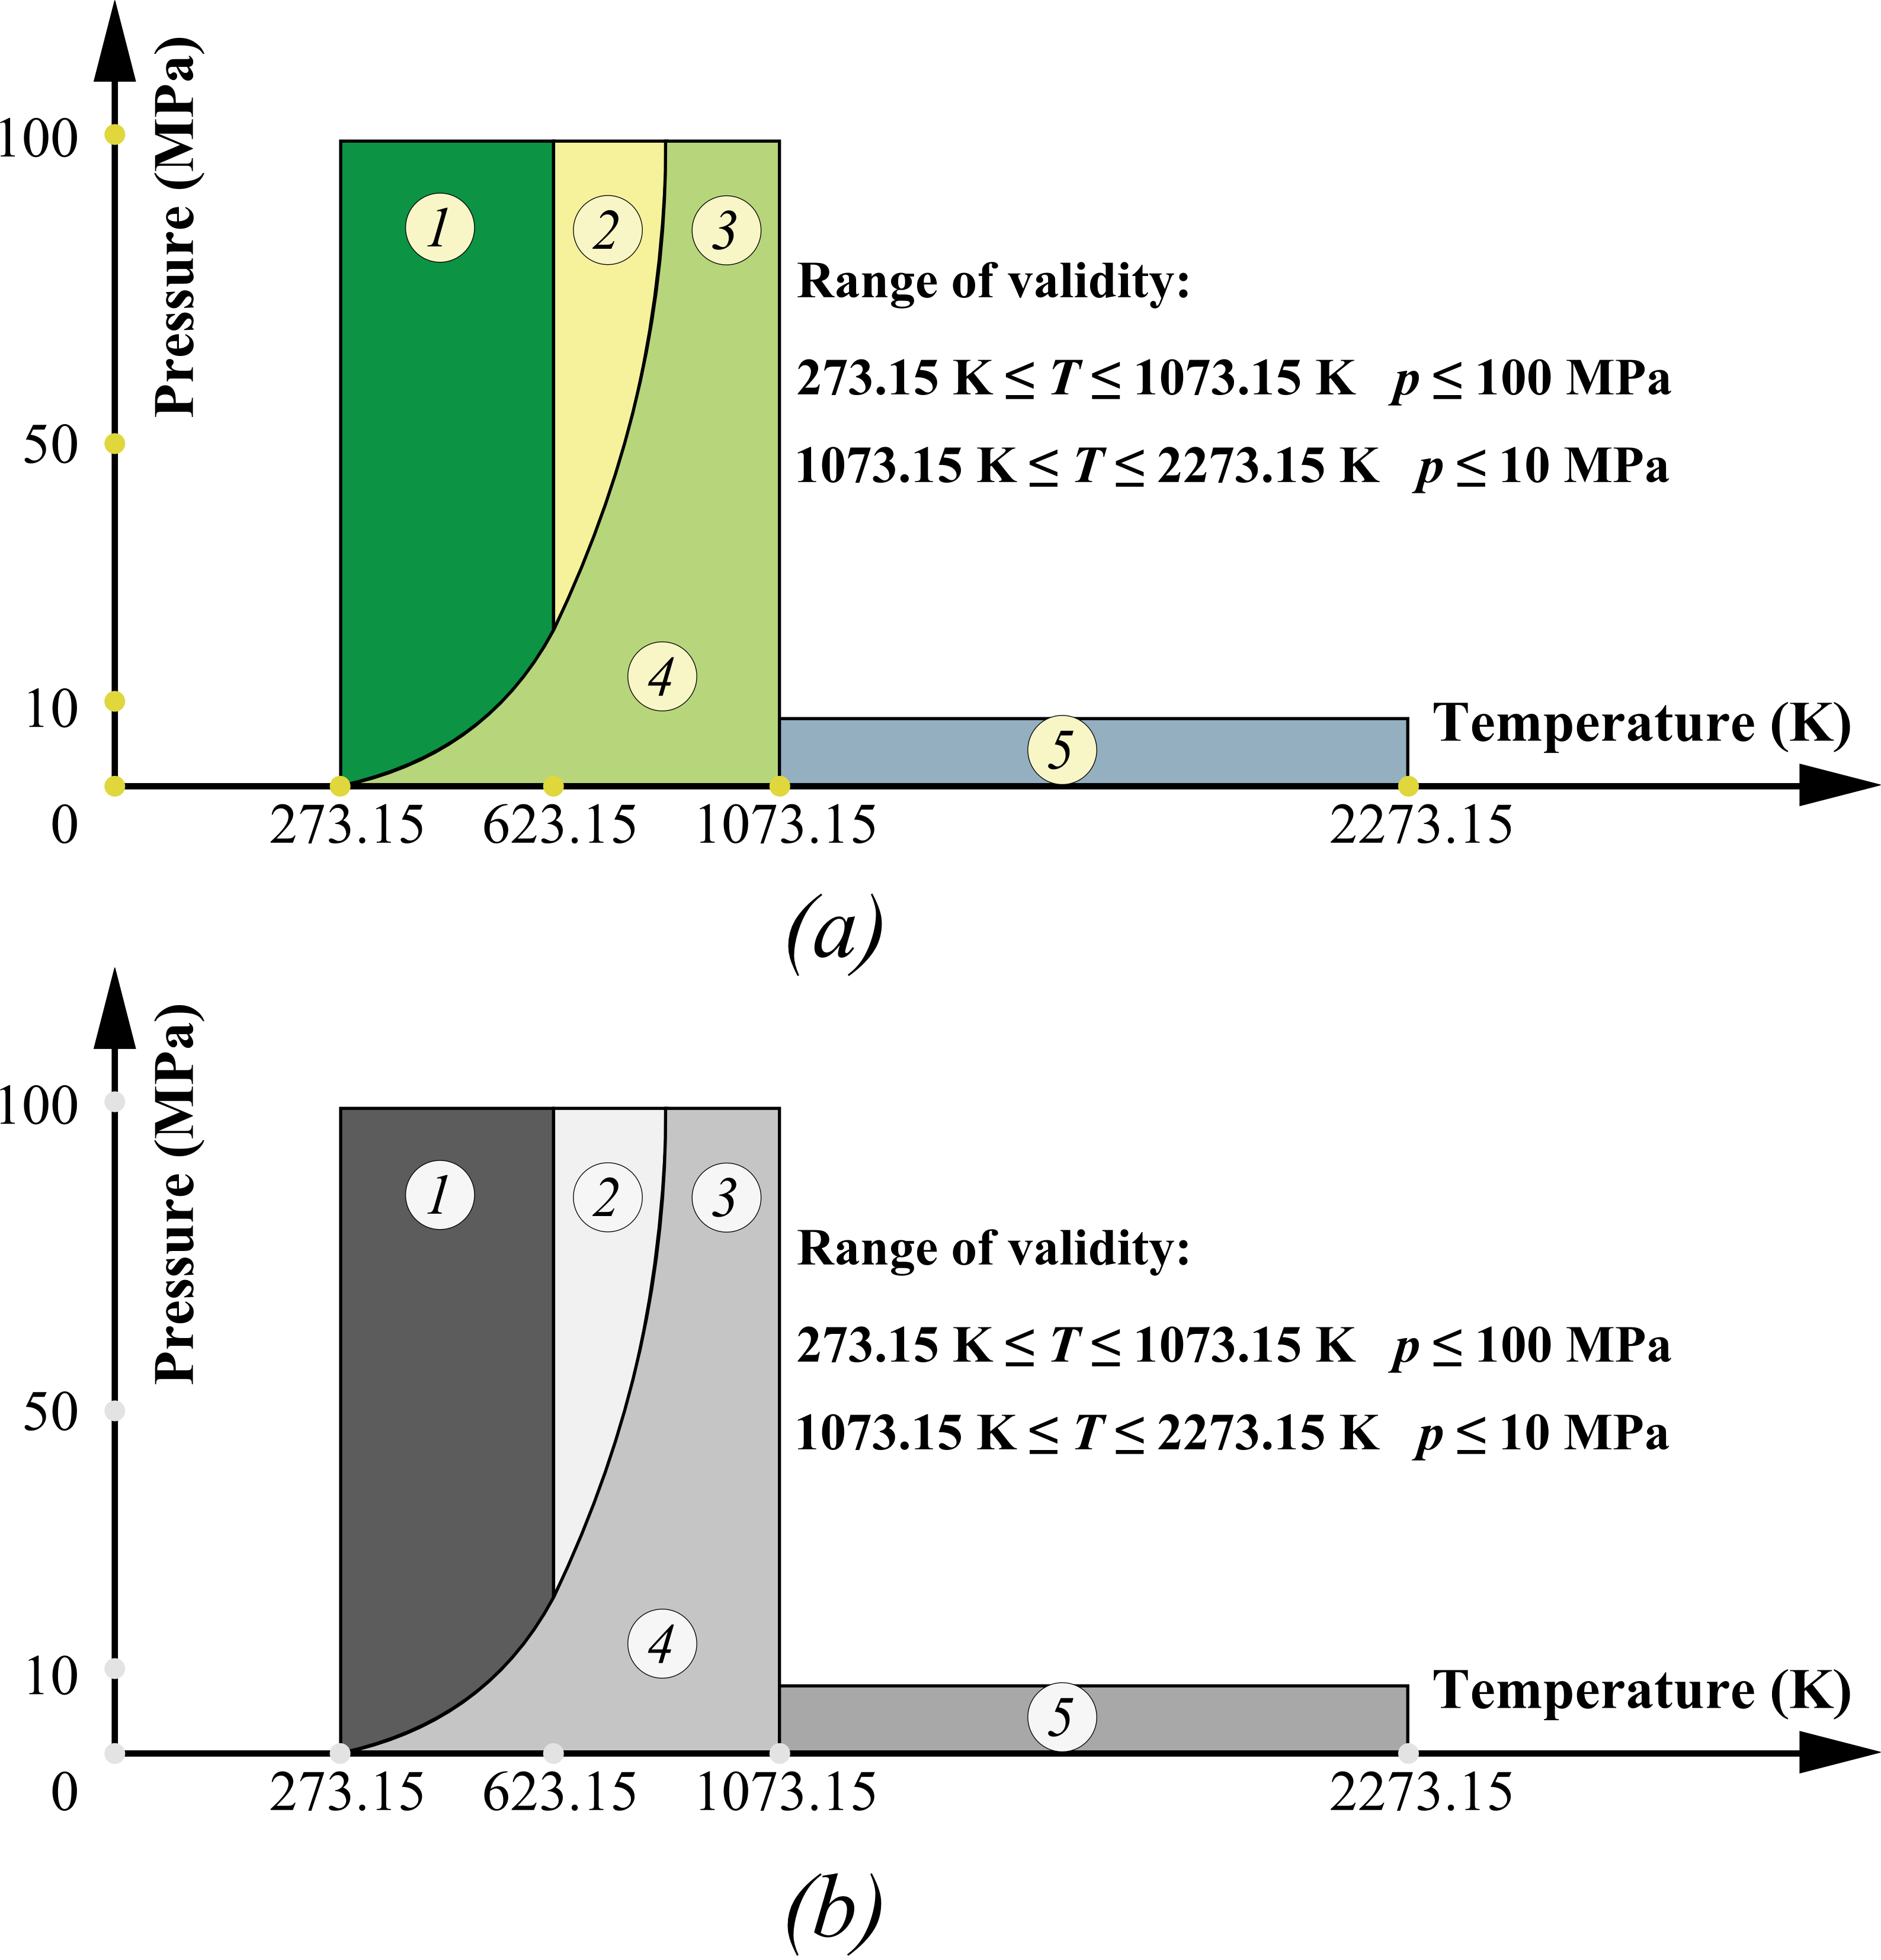
\includegraphics{Figure_1.png}
    \caption{Use of appropriate contrasted colours for black and white printing: a) colour figure, b) greyscale figure.}
    \label{Fig_1}       % Give a unique label
\end{figure}

Before inserting in the document each figure should be:

\begin{itemize}
    \item Prepared as simply as possible for clarity. Avoid sideways illustrations if possible.
    \item Sized to the desired final dimensions in order to minimize the final document file size.
    \item Prepared with at least 300 dpi resolutions for raster artwork (greyscale and colour halftones), 600 dpi for combinations (line art and halftone together) and 1200 dpi for line art.
\end{itemize}

To embed (insert) images, prepared in separate files, authors should use \textit{figure} environment. If the authors are providing scanned figures, they have to be clear, with all the legends and data labels easily readable. If this is not possible, the author must redraw the figures especially in the case of simple ones. Illustrations borrowed or adapted from another source have to be properly acknowledged. Figure caption should be below the figure.

When a figure is referred to in the text, it should be typed as Fig \ref{Fig_1} or Figs 2 to 4, with ``Fig." capitalized and abbreviated (unless it is the first word in a sentence) and without period at the end (unless the reference appears at the end of a sentence).

\sffamily \subsubsection{Tables} \label{Tables}
\rmfamily
All tables should be prepared using \textit{table} environment. Tables should be numbered consecutively and captioned, the caption should be 10pt Roman, upper and lower case letters. Table caption should be above the Table.

Tables should be as simple as possible, with single horizontal lines above and below column headings and subheadings, and at the bottom of the table (if it is necessary the authors may put horizontal lines between the rows). Limit the number of columns to fewer than 10, since the use of many columns will create readability problems. Vertical lines and shaded areas should be avoided where possible. Fancy frames or borders around tables should not be used.

\begin{table}[h]
\caption{Table format in ECOS: Template for manuscripts}
\begin{center}
\begin{tabular}{*{4}{c}}
\hline
Month & $\rho_{cs}$, \% & $\rho_{ps}$, \% & $\rho_{os}$, \%\\
\hline
JAN & 5.88 & 36.88 & 57.24 \\
FEB & 6.79 & 45.65 & 47.57 \\
MAR & 5.48 & 40.40 & 54.12 \\
APR & 16.39 & 51.58 & 32.03 \\
MAY & 11.18 & 45.27 & 43.55 \\
JUN & 12.87 & 33.68 & 53.45 \\
JUL & 15.94 & 40.45 & 43.62 \\
AUG & 6.10 & 50.22 & 43.68 \\
\hline
\end{tabular}
\end{center}
\label{Table_1}
\end{table}

When Tables are referred to in the text, they should be typed as Table \ref{Table_1} or Tables 2 to 4. Authors should not abbreviate ``Table" and should not put period after number, unless the reference appears at the end of a sentence.

\sffamily \Large \section*{Acknowledgments}
\rmfamily \normalsize
Any acknowledgments authors wish to make should be included in a separate section with normal formatting, at the end of the main text and before the appendix (if any), nomenclature and references section. This section starts with headings Acknowledgments.

\sffamily \Large \section*{Appendix}
\rmfamily \normalsize
An Appendix, if needed, should appear after the acknowledgments.

\sffamily \Large \section*{ Nomenclature}
\rmfamily \normalsize
If symbols are used extensively, paper must have a separate Nomenclature section. Section starts with a heading Nomenclature. This section lists in detail all the symbols used in the text and their definitions. The list should include:
%
\begin{itemize}
    \item Letter symbol; each symbol used in a paper should have a unique definition.
    \item Accurate and concise definition of symbol. Definitions do not require ''the'' and are followed by comma and one space.
    \item Units of measure used in the paper. No end punctuation in nomenclature.
\end{itemize}
%
All Letter symbols (dimensional and dimensionless) should be listed in an alphabetic order. Letter symbols are followed by Greek symbols, subscripts and superscripts.

%\begin{nomenclature}
%    \item[$\dot m_k$]   stream of $k$-th harmful substance leaving balance boundary of power unit,
%    \item[$N_{el}$] net electric power but not with concentration,
%    \item[$P_{k,el}$] amount of $k$-th harmful substance burdening the production of electricity.
%\end{nomenclature}
\vspace{6pt}
\textbf{Example}
\begin{description}[leftmargin=!,labelwidth=\widthof{maxlength}]
    \item[$c$] specific heat, ${\rm J/(kgK)}$
    \item[$h$] heat transfer coefficient, ${\rm W/m^{2}K}$
    \item[$\Dot{m}$] mass flow rate, ${\rm kg/s}$
    \item[$t$] temperature, ${\rm ^\circ C}$
\end{description}

\textbf{Greek symbols}
\begin{description}[leftmargin=!,labelwidth=\widthof{maxlength}]
    \item[$\eta$] efficiency
    \item[$\phi$] maintenance factor
\end{description}

\textbf{Subscripts and superscripts}
\begin{description}[leftmargin=!,labelwidth=\widthof{maxlength}]
    \item[a] Air
\end{description}

\sffamily \large \subsection{Citations}
\rmfamily \normalsize
Authors should acknowledge the reference sources (either from a printed document or from the web) whenever they:
%
\begin{itemize}
    \item Paraphrase or summarize another person's ideas or points.
    \item Quote another person's work.
    \item Use information from any source, including information contained in tables, graphs, figures or diagrams.
\end{itemize}
%
ECOS uses the numeric system of referencing, according to the conventions set down in the Vancouver/Numeric style. References to cited literature should be numbered consecutively throughout the paper and collected together in a section References.
In the text, each reference number (Arabic numerals) should be enclosed in square brackets in the same line as the text (\cite{journal}, \cite{proceedings}), before any punctuation such as: full stops, commas, colons and semi-colons. Author should refer to the reference number, and do not use ``Ref. \cite{chapter}" or ``reference \cite{chapter}" except at the beginning of a sentence: ``Reference \cite{chapter} was..." When multiple references are cited at a given place in the text, author should:
%
\begin{enumerate}
    \item Use a hyphen to join the first and last numbers that are inclusive: \cite{proceedings,chapter,books,report}.
    \item Use commas (without space) to separate no inclusive numbers in a multiple citation \cite{proceedings,chapter,books,report, web_references}.
\end{enumerate}
%
A reference to a particular article or chapter in a book may be cited in the text multiple times but must only appear once in the reference list. During the text preparation authors are encouraged to:
\begin{itemize}
    \item Substitute reference numbers for the name of the author whenever appropriate:
    \begin{itemize}
        \item As Smith, Wesson and Ruger, and Williams et al. demonstrate, {\bf incorrect}.
        \item As \cite{journal}, \cite{proceedings}, and \cite{chapter} demonstrate, {\bf correct}.
        \item As Smith \cite{journal}, Wesson and Ruger \cite{proceedings}, Williams et al. (for more than 2 co-authors) \cite{chapter}.{\bf correct}.
    \end{itemize}
    \item Place numbers directly after the reference rather than at the end of a clause or sentence, (unless the reference ends at the end of a clause or sentence).
    \begin{itemize}
        \item One study examined the energy efficiency in ... \cite{journal}, {\bf incorrect}.
        \item One study \cite{journal} examined the energy efficiency in ...., {\bf correct}.
    \end{itemize}
\end{itemize}

Authors must provide a full description of each source which has been cited in the text in a references list. The information must be sufficient to make it possible for interested readers to easily locate and obtain the source. The references should be listed in the same order as cited in the text, not in alphabetical order.

References to electronic data available only from personal Web sites or commercial, academic, or government ones where there is no commitment to archiving the data, should be avoided. Depending on the circumstances, private communications, Web site addresses, citations like ``In preparation" and ``To be submitted" may be incorporated into the main text of a paper or may appear in appendix. The following examples demonstrate the format for a variety of types of references.

Citations should be given according to the examples in the section References for articles in journals \footnote{Journal titles can be abbreviated, see URL: http://www.efm.leeds.ac.uk/~mark/ISIabbr/.} \cite{journal}, \cite{journal2} and proceedings \cite{proceedings}, chapter in book \cite{chapter} as well as for books \cite{books}, technical reports \cite{report}, dissertations \cite{dissertation} and web available sources \cite{web_references}.

\sffamily \Large
% \begin{thebibliography}{99}
\rmfamily \normalsize
\bibliographystyle{plain}
\bibliography{energy_storage}
% \end{thebibliography}

\end{document}
